\newcommand{\svcourse}{CST Part IA: Introduction to Probability}
\newcommand{\svnumber}{1}
\newcommand{\svvenue}{Churchill, Room TBD}
\newcommand{\svdate}{2022-05-14}
\newcommand{\svtime}{11:00}
\newcommand{\svuploadkey}{PO5ogKIM8KQA22FZS8IAf8gxA8XKi19jxIBVHIfFZ+3GCBXuNUXS9lVN6bNYjxM/}

\newcommand{\svrname}{Mr Matthew Ireland}
\newcommand{\jkfside}{twoside}
\newcommand{\jkfhanded}{right}

\newcommand{\studentname}{Harry Langford}
\newcommand{\studentemail}{hjel2@cam.ac.uk}


\documentclass[10pt,\jkfside,a4paper]{article}

% DO NOT add \usepackage commands here.  Place any custom commands
% into your SV work files.  Anything in the template directory is
% likely to be overwritten!

\usepackage{fancyhdr}

\usepackage{lastpage}       % ``n of m'' page numbering
\usepackage{lscape}         % Makes landscape easier

\usepackage{verbatim}       % Verbatim blocks
\usepackage{epsfig}         % Embed encapsulated postscript
\usepackage{array}          % Array environment
\usepackage[nolinks]{qrcode}         % QR codes
\usepackage{enumitem}       % Required by Tom Johnson's exam question header

\usepackage{hhline}         % Horizontal lines in tables
\usepackage{siunitx}        % Correct spacing of units
\usepackage{amsmath}        % American Mathematical Society
\usepackage{amssymb}        % Maths symbols
\usepackage{amsthm}         % Theorems

\usepackage{ifthen}         % Conditional processing in tex

\usepackage[top=3cm,
            bottom=3cm,
            inner=2cm,
            outer=5cm]{geometry}

% PDF metadata + URL formatting
\usepackage[
            pdfauthor={\studentname},
            pdftitle={\svcourse, SV \svnumber},
            pdfsubject={},
            pdfkeywords={9d2547b00aba40b58fa0378774f72ee6},
            pdfproducer={},
            pdfcreator={},
            hidelinks]{hyperref}

\renewcommand{\headrulewidth}{0.4pt}
\renewcommand{\footrulewidth}{0.4pt}
\fancyheadoffset[LO,LE,RO,RE]{0pt}
\fancyfootoffset[LO,LE,RO,RE]{0pt}
\pagestyle{fancy}
\fancyhead{}
\fancyhead[LO,RE]{{\bfseries \studentname}\\\studentemail}
\fancyhead[RO,LE]{{\bfseries \svcourse, SV~\svnumber}\\\svdate\ \svtime, \svvenue}
\fancyfoot{}
\fancyfoot[LO,RE]{For: \svrname}
\fancyfoot[RO,LE]{\today\hspace{1cm}\thepage\ / \pageref{LastPage}}
\fancyfoot[C]{\qrcode[height=0.8cm]{\svuploadkey}}
\setlength{\headheight}{22.55pt}

\ifthenelse{\equal{\jkfside}{oneside}}{

 \ifthenelse{\equal{\jkfhanded}{left}}{
  % 1. Left-handed marker, one-sided printing or e-marking, use oneside and...
  \evensidemargin=\oddsidemargin
  \oddsidemargin=73pt
  \setlength{\marginparwidth}{111pt}
  \setlength{\marginparsep}{-\marginparsep}
  \addtolength{\marginparsep}{-\textwidth}
  \addtolength{\marginparsep}{-\marginparwidth}
 }{
  % 2. Right-handed marker, one-sided printing or e-marking, use oneside.
  \setlength{\marginparwidth}{111pt}
 }

}{
 % 3. Alternating margins, two-sided printing, use twoside.
}

\setlength{\parindent}{0em}
\addtolength{\parskip}{1ex}

% Exam question headings, labels and sensible layout (courtesy of Tom Johnson)
\setlist{parsep=\parskip, listparindent=\parindent}
\newcommand{\examhead}[3]{\section{#1 Paper #2 Question #3}}
\newenvironment{examquestion}[3]{
    \examhead{#1}{#2}{#3}\setlist[enumerate, 1]{label=(\alph*)}\setlist[enumerate, 2]{label=(\roman*)}
    \marginpar{\qrcode{https://www.cl.cam.ac.uk/teaching/exams/pastpapers/y#1p#2q#3.pdf}}
    \marginpar{\footnotesize \url{https://www.cl.cam.ac.uk/teaching/exams/pastpapers/y#1p#2q#3.pdf}}
}{}



\usepackage{float}
\usepackage{tikz}

\begin{document}

\begin{enumerate}

\item What advantage does a single virtual address space design offer over
traditional unix-style multiple virtual address spaces?

Using a single virtual address space means that all processes have access to
all addresses in the system. Therefore we do not have to flush or invalidate
cache or TLB on context switches or load a new page table. This makes context
switches to processes which do not use much memory or are short-lived very
cheap -- when we context switch back the cache will be largely untouched.
This could significantly speed up execution on a system executing lots of
processes concurrently. Consider a system running two processes: a CPU-bound
process which uses a lot of memory and an I/O bound process. When the I/O
bound process unblocks we can context switch to it, deal with the I/O and
make another blocking request if necessary and then context switch back to
the CPU bound process. Since very little data was used by the I/O task, the
cache is largely unaffected -- meaning the CPU process does not need to
refill the cache from RAM or disk and therefore the overhead of the context
switches was significantly less than if we had used unit-style multiple
address spaces.

\item

\begin{examquestion}{2004}{6}{2}

the ARM processor allows the second operand to be shifted by an arbitrary
amount. In order to improve the performance, a six-stage pipeline is
proposed with the following stages:

\begin{table}[H]
\centering
\begin{tabular}{|c|c|c|c|c|c|}
\hline
instruction & decode and & shift & execute & memory & register \\
fetch & register fetch & operand 2 & & access & write back \\
\hline
\end{tabular}
\end{table}

\begin{enumerate}[label=(\alph*)]

\item What are control hazards and how could they be resolved in the above
pipeline?

Between the time a branch instruction is issued and leaves the execute
stage, the processor cannot determine what the next instruction to be issued
should be. This is known as a Control Hazard.

There are three ways we can help resolve Control Hazards in the above pipeline:

\begin{itemize}

\item Write back to the PC in the Execute stage

In the above pipeline, whether a branch is taken or not and the destination
of that branch is known at the end of the execute stage. However, the PC is
only updated two stages later in the register write-back stage. If we write
to the PC in the execute stage, then we can reduce the branch delay slot by
1 (to 4 cycles) and make other strategies more efficient.

\item Issue NOPs

After we issue a branch, we can fill the branch delay slot with NOPs. This
means that no instruction is executed until we know the result of the branch
and therefore guarantees correctness. However this means we waste cycles
issuing NOPs.

\item Execute Speculatively

After issuing a branch, the processor can predict whether the branch will be
taken or not and the likely target of the branch. We can then issue
instructions from this address and execute them speculatively. If our guess
is correct then we improve performance; and if our guess was incorrect then
 we can abort the speculative instructions before they take effect.

\end{itemize}

In a pipeline as shallow as the example, I believe the best strategy would
be to issue 3 NOPs and write back to the program counter (or add a
forwarding path) after the execute stage so that the branch delay slot was 4
cycles and then issue 4 NOPs. This strategy would become unsuitable for
deeper pipelines.

\item What are data hazards and how could they be resolved in the above
pipeline?

A data hazard is a conflict between two instructions. A data hazards arises
when one instruction modifies a register but has not yet committed the new
value before the second instruction attempts to fetch the uncommitted
register. The second instruction therefore cannot complete correctly as it
cannot access the correct value of its operand.

The data hazards in the above pipeline are shown by dashed lines in the
diagram below:

\begin{center}
\begin{tikzpicture}
\node[anchor=center] at (0, 0.4) {Instruction Fetch};
\node[anchor=center] at (0, -0.6) {Decode and};
\node[anchor=center] at (0, -1) {Register Fetch};
\node[anchor=center] at (0, -2) {Shift Operand 2};
\node[anchor=center] at (0, -3) {Execute};
\node[anchor=center] at (0, -4) {Memory Access};
\node[anchor=center] at (0, -5) {Register Write-back};
\draw[-stealth] (0, 0.15) -- (0, -0.35);
\draw[-stealth] (0, -1.25) -- (0, -1.75);
\draw[-stealth] (0, -2.25) -- (0, -2.75);
\draw[-stealth] (0, -3.25) -- (0, -3.75);
\draw[-stealth] (0, -4.25) -- (0, -4.75);

\draw[-stealth, dashed] (-0.2, -3.25) -- (-0.2, -3.5) -- (-1.5, -3.5) --
(-1.5, -2.5) -- (-0.2, -2.5) -- (-0.2, -2.75);
\draw[-stealth, dashed] (-1.5, -2.5) -- (-1.5, -1.5) -- (-0.2, -1.5) --
(-0.2, -1.75);
\draw[-stealth, dashed] (-1.5, -1.5) -- (-1.5, -0.1) -- (-0.2, -0.1) --
(-0.2, -0.35);

\draw[-stealth, dashed] (0.2, -4.25) -- (0.2, -4.5) -- (1.5, -4.5) --
(1.5, -3.5) -- (0.2, -3.5) -- (0.2, -3.75);
\draw[-stealth, dashed] (1.5, -3.5) -- (1.5, -2.5) -- (0.2, -2.5) --
(0.2, -2.75);
\draw[-stealth, dashed] (1.5, -2.5) -- (1.5, -1.5) -- (0.2, -1.5) --
(0.2, -1.75);
\draw[-stealth, dotted] (1.5, -1.5) -- (1.5, -0.1) -- (0.2, -0.1) --
(0.2, -0.35);
\end{tikzpicture}
\end{center}

Each dashed line indicates a possible data hazard. The origin of the line
indicates the first point at which the updated value would be known and the
destination of the line indicates where it would be needed.

Notice the dotted line between Memory Access and Decode and Register Fetch.
This is because this could be a data hazard, but a very common optimisation
is to write in the first half of the clock cycle and read from the second.
This means that in practice this is not problematic.

We can add feed-forward paths where each of the dotted lines are in order to
resolve most data hazards.

Note that these feed-forward paths would not solve every data hazard. There
are three cases which feed forward paths cannot solve:

\begin{itemize}

\item Storing the result of execute in a register where this register is the
operand being shifted in the next instruction or the amount by which
operand 2 is being shifted. This causes a bubble of size 1.

\item Storing the result of a memory access in a register and one of the
next two instructions is the operand being shifted or the amount by which
operand 2 is being shifted. This causes a bubble of size 2.

\item Storing the result of a memory access in a register and immediately
using it as an operand in the next execute. This data hazard causes a bubble
of 1 cycle.

\item Latency by memory access -- memory accesses can take significantly
more than 1 cycle -- the latency caused by memory access and potential
solutions to that is a separate topic which I discussed thoroughly in the
last supervision.

\end{itemize}

\item What are feed-forward paths and where could they be added to the above
pipeline to improve performance?

Feed-forward paths are wires which can send data to earlier pipeline stages
before the data has been written. This reduces the number of pipeline
bubbles caused by certain instructions. These wires (along with appropriate
control signals) go into a multiplexor with the operands from the previous
stage. If one of them comes from the register which has just been written
to, then the control signal makes the multiplexer output the modified value.

\item Why might a branch instruction result in pipeline bubbles and how many
bubbles will appear in the above pipeline as a result of taking a branch
instruction?

If a branch instruction is issued then the processor cannot determine which
instruction it should issue until the branch is partially executed. One
way to resolve this is to issue \textit{no instructions} until the branch
writes back to the program counter.

Dependent on the type of branch, the number of pipeline bubbles will be
different:

\begin{itemize}

\item Conditional branches will cause four pipeline bubbles. Conditional
branches require arithmetic to determine whether the branch will be taken.
Therefore the processor cannot determine the next instruction until after
the execute stage.

\item Unconditional branches which require arithmetic such as JALR will
cause four pipeline bubbles. The processor cannot determine the address of the
jump (and the next instruction) until after arithmetic has been performed in
the execute stage.

\item Unconditional branches by constant amounts or register-amounts will
cause two pipeline bubbles. The processor can determine the next instruction
after the immediate from the instruction is decoded -- at the start of the
execute stage.

\end{itemize}

\end{enumerate}

\end{examquestion}

\item Using your summer work as a starting point, describe what each of the
following terms mean and why it is important to CPU cache design (hint: for
each principle of cache design, give an example use case when it is very
appropriate and when it is very inappropriate)

\begin{enumerate}[label=(\alph*)]

\item A write-back policy

Under a write-back policy, we only write to the lowest cache in which the
data is stored (L1 being the lowest possible and RAM being the highest). We
add a ``dirty bit'' to each cacheline which states whether the cacheline has
been written to since it was loaded in. On writing, we set the dirty bit to
1 and update the value. We critically do not write to higher-level caches.
This leaves caches in an inconsistent state. Before we make a cacheline a
victim, we may have to write it into a higher level cache. This means
victimisation is slower but writes are faster.

This is very good when we perform a lot of updates on a small set of data.
It means we only have to update values in L1 cache rather than L1, L2, L3
and RAM . Consider the following C code. In a write-back cache, the updates
to $i$ and $n$ only involve writing to L1 cache. Write-back significantly
reduces the number of writes and dramatically speeds up cache speed on
multicore systems if cores are operating on different addresses.

\begin{lstlisting}[language=C]
int main(void){
	int n = 0;
	for (int i = 0; i < 100; i++){
		n += i;
	}
}
\end{lstlisting}

However, write-back caches are \textit{very} bad for cache consistency and
add significant complexity on multicore systems. If we have multiple cores
which are accessing shared data, then if a core wants to access any data we
can only fetch from a higher level cache if we know the data is not stored
in any \text{other cores caches}. This is commonly implemented using a
``snoopy bus'' where each core ``snoops on'' (sees) the read and write
requests from all other cores. If any other core requests data stored in
cache or the write buffer, it is marked as invalid in cache and sent to the
other core. Simpler implementations (ARM writes the write buffer out) will
write the cache or write buffer entry out into the higher level cache and
stall the read request. More advanced implementations can have access rights
on cache and allow shared read-only copies of data. This adds a lot of
additional complexity and scales poorly for large numbers of cores.

\item A write-through policy

Under a write-through policy, all writes will write to all higher levels of
cache -- so a write to L1 cache will write to L1, L2, L3 and RAM. This makes
writes very slow and adds a lot of traffic on the data bus.

Write-through is good for cache consistency -- we don't need to write to
higher level caches when evicting cachelines or switching threads. The hardware
required is simpler -- we don't need a dirty bit or to consider writing back
when victimising cache. We can buffer writes using the write buffer meaning
that if we infrequently make writes, the CPU will not stall on writes --
hence making the common case fast. Write-through is therefore appropriate on
simpler systems.

Write-through has very bad performance if we update values a lot (assuming we
are not write-merging) -- we would do a lot of writes and they will all be
immediately overwritten. Consider bubblesorting a medium-length array of
length $n$. Since we change variables $O(n^2)$ times, there will be
$O(n^2)$ writes back to RAM under write-through -- while under write-back we
would update the values in cache and so would only have to write back the
final value -- $O(n)$ writes to higher memory.

\item A write-around policy

Under a write-around policy if we attempt a write to memory which is not in
L1 cache, the CPU will write into the lowest cache or memory in which
the address is stored without loading the address into any lower caches.

This has the advantage of not polluting the cache with dead data which we
never intend to write to.

However, if we initialise a variable and attempt to read from it later
then the variable will not be in cache and therefore we will have to access
RAM . So under write-around we have to access RAM twice for most variables
we initialise. Notice that if we write and then immediately read then the
value of the variable may still be in the write-buffer -- however this case
is rare and so most CPUs do not implement hardware for fetching from the
write buffer. In this case we will write the write buffer out to memory and
then fetch from memory -- meaning the CPU needs to wait for 3 memory accesses
rather than just 1!

\iffalse

However, write-around makes cache coherency \textit{very} challenging
and so the disadvantages strongly outweigh the advantages on a single-core
system. Consider if one core writes to an address in main memory and while
this write is still in the first cores write-buffer, a second core attempts to
read this value.

Write-around is particularly efficient with a large write buffer -- if the
write-buffer is large then the amount of write calls which block is greatly
reduced. Similarly, write-merge works well with write-around -- most of the
time when we are writing to data without reading it we are writing to large
blocks of contiguous data -- such as a memcopy, initialising an array or
filling a framebuffer. Write-merging (specifically merging adjacent writes
into a single write) can reduce the number of writes we significantly.

However, almost all variables are initialised before use. Therefore
whenever we initialise any variable (except for array-like data structures),
we will have to perform two memory accesses -- one to write and initialise
and a second to load the value.

Write-around gets poor performance if we initialise values immediately
before use as we will have to do two memory accesses for the same data.

I thought about the advantages and disadvantages of write-around cache a lot.
I'm fairly sure it's only advantageous if used in conjunction with
write-merging. If we use it without write-merging then we take no advantage
of spatial locality and so zeroing an array would take 4--16x more memory
accesses than if we loaded the array cacheline-by-cacheline into cache.
This massive memory access overhead surely outweighs any advantage related
to ``keeping cache clean'' -- 80\% of cache is ``dead data'' and so refilling
cache would take less time than the 4--16x additional memory access overhead.
The set of cases write-around is efficient without write-merging feels
niche: we need to have no spatial or temporal locality -- writing to a set of
unrelated data without subsequently reading from them isn't an operation CPUs
do frequently. If used in conjunction with write-merging then write-allocate
will dramatically speed up array initialisation -- and marginally slow
almost everything else down. Given the dramatic additional complexity and
lack of cache consistency due to write-merging, it feels like an
optimisation that is not worthwhile. On multiple cores, if we use
write-merging we have to check not only every cache, but also every write
buffer for each core for any shared cache access.

\fi

\item A victim buffer

A victim buffer is a very small cache which contains the most recently
evicted cachelines. On cache misses, we first look in the victim buffer
associatively to see if the cacheline we want is stored there. If so we swap
it back in. Victim buffers are typically 1--4 cachelines large.

Victim buffers are particularly useful in direct-mapped caches -- direct
mapped caches have no choice in which cacheline to evict and therefore
frequently evict cachelines which are currently in use. Adding a victim
buffer reduces the impact of this -- rather than looking in higher-level
caches the result is likely in the victim buffer.

In associative caches, victim buffers are useless. Associative caches have
no restrictions on where cachelines can be places and therefore have great
freedom over which cacheline to evict. So associative caches have proper
eviction algorithms and can determine the optimal choice of cachelines
to evict. Adding a victim buffer is the same as slightly increasing the size
of the associative cache -- and accessing this new section serially. This
provides no benefit and only slows down cache fetches.

\item write-merging/combining/collapsing/coalescing

Under write-merging we will merge adjacent writes or multiple writes into the
same memory address into a single write. Write-merging can reduce the
total number of writes performed. This merging is done in the write buffer
and can speed up operations such as an array initialisation or a
memcopy.

Writing to memory is one of the bottlenecks of processors and so
significantly reducing the number of writes dramatically increases
performance. Write-merging is particularly good if we are writing large
contiguous blocks into memory which we do not subsequently read from (hence
do not require strong ordering and so we do not add overhead to other reads).
This makes write merging particularly useful for GPUs.

However, write-merging requires us to stall writes into higher level caches
to check for later writes that can be merged. Therefore writes may take
significantly longer and cache coherency becomes harder on multicore systems.
On modern processors which support write-merging, order guarantees are not
made.

Write-merging cannot be used in conjunction with write-around. If it was
then on every read, the data could be in the write buffer. Therefore the
processor would either have to use the write-buffer like an associative
cache or flush the write buffer on every read. Both add significant
overhead. This problem is exemplified on multiple cores where any read from
any core would have to look in or flush every write buffer.

\item A virtually-addressed cache

In a virtually addressed cache, the cache is addressed by virtual addresses.
Therefore, we only have to do TLB lookups on cache misses. However we must
flush (or invalidate) the cache on context switches since virtual addresses
are not globally unique. This decreases the overhead of cache lookups but
increases the overhead of context switches.

Virtually addressed caches are suitable when performing CPU-bound tasks --
these tasks benefit from low memory access costs and are not significantly
affected by a small increase in the overhead of a context switch.

Virtually addressed caches are less suitable when performing IO-bound tasks --
these tasks are loaded in (forcing the CPU to flush or invalidate the
cache), perform a small number of instructions and then return leaving the
cache invalidated.

\item A physically addressed cache

In physically addressed cache, the cache uses physical addresses. However,
the program still uses virtual addresses. Therefore, we need to do a
virtual-to-physical translation before cache accesses. 99.8\% of the time
this is a single TLB access -- however sometimes this will involve
loading in a new page table which will add significant overhead.

Using physically addressed cache means we do not need to invalidate cache on
context switches. This reduces the overhead of multiprocessing.

However, the additional overhead from virtual-to-physical translations
before every cache access is significant.

\item Cache coherency

Cache coherency is a property which multicore systems aim to achieve. Cache
coherency means that any set of cores reading the same address from memory
at the same time guaranteed to all read the same value. This is a difficult
property to preserve especially with CPU optimisations such as
write-buffering or write-merge. However, Cache Coherency is essential to
implement multicore systems without race conditions.

Cache Coherency is very good for general-purpose multicore systems. It
allows multiple cores to operate on shared data and execute correctly
without race conditions.

However, Cache Coherency is not suitable for GPUs -- the principle of a GPU
is to maximise the time spent executing independent arithmetic operations. In
GPUs different cores should not generally be reading from data that other
cores have written to. Implementing Cache Coherency would for GPUs would
significantly increase overhead and allow GPUs to perform operations they
are not designed to.

\item A cacheline dirty bit

Cacheline dirty bits indicate that the cacheline has been written to. This
means that if we evict the cacheline then we must write it back -- and if
the dirty bit is not set then we do not have to write back. This speeds up
execution time as we don't have to write back read-only memory and can also
implement a write-back policy.

However, dirty bits are made redundant by multicore protocols like MSI .
Under MSI, cachelines are in one of three states: modified, shared or
invalid. If a cacheline is in the modified state then it must be written
back on eviction otherwise it does not. This is a strict superset of the
control that dirty bits provide. Therefore any processor using the MSI
protocol does not need to have dirty bits.

\item Direct-Mapped Caching

With Direct-Mapped caching, each cache has a hash function which maps an
address in memory to an address in the cache. These hash functions are
generally simple -- such as bits [4--16] of the address. Therefore we can
very quickly find where the data will be stored in cache if it is in cache.
Direct-Mapped caches are very simple and very fast.

However, if we want to load new data into cache then there is only one place
in which to store it. This may conflict with other data we are using and
force us to evict data we are actively using; which can lead to pathologically
bad cases. This can be mitigated by the use of a victim buffer.
As a result, Direct-Mapped Caches have lower cache quality.

\item Set-Associative Caching

In $n$-way Set Associative Caching, the cache is partitioned into $n$
sets (each of which can be used like a Direct-Mapped Cache). Therefore we can
use a hash function and check the location in each of the $n$ sets in
parallel. $n$ is much smaller than the total number of cachelines in the
cache (8--16 is typical) and therefore is much faster than Associative
caches. There are now $n$ locations in which a particular cacheline can be
placed and so we can run cache replacement algorithms -- such as ``Least
Recently Used'' or ``Not Last Used'' to determine which of the $n$
cachelines to evict. These algorithms help ensure high cache quality.

\end{enumerate}

\end{enumerate}

\end{document}
